%
% Niniejszy plik stanowi przykład formatowania pracy magisterskiej na
% Wydziale MIM UW.  Szkielet użytych poleceń można wykorzystywać do
% woli, np. formatujac wlasna prace.
%
% Zawartosc merytoryczna stanowi oryginalnosiagniecie
% naukowosciowe Marcina Wolinskiego.  Wszelkie prawa zastrzeżone.
%
% Copyright (c) 2001 by Marcin Woliński <M.Wolinski@gust.org.pl>
% Poprawki spowodowane zmianami przepisów - Marcin Szczuka, 1.10.2004
% Poprawki spowodowane zmianami przepisow i ujednolicenie 
% - Seweryn Karłowicz, 05.05.2006
% dodaj opcję [licencjacka] dla pracy licencjackiej
\documentclass{pracamgr}

\usepackage{polski}

%Jesli uzywasz kodowania polskich znakow ISO-8859-2 nastepna linia powinna byc 
%odkomentowana
%\usepackage[latin2]{inputenc}
%Jesli uzywasz kodowania polskich znakow CP-1250 to ta linia powinna byc 
%odkomentowana
\usepackage[utf8]{inputenc}
\RequirePackage{graphicx}
\RequirePackage{longtable}
\usepackage[usenames,dvipsnames]{color}
%\usepackage{hyperref}
%\usepackage{url}
\definecolor{gray}{RGB}{50,50,50}

\usepackage[colorlinks=true,linkcolor=gray,urlcolor=blue]{hyperref}  



\newcommand{\emptyP}{\mbox{$\epsilon$}}
\newcommand{\terminal}[1]{\mbox{{\texttt {#1}}}}
\newcommand{\nonterminal}[1]{\mbox{$\langle \mbox{{\sl #1 }} \! \rangle$}}
\newcommand{\arrow}{\mbox{::=}}
\newcommand{\delimit}{\mbox{$|$}}
\newcommand{\reserved}[1]{\mbox{{\texttt {#1}}}}
\newcommand{\literal}[1]{\mbox{{\texttt {#1}}}}
\newcommand{\symb}[1]{\mbox{{\texttt {#1}}}}
% Dane magistranta:

\author{Imię i nazwisko}

\nralbumu{nralbumu}

\title{Intuicyjny język wyszukiwania TQL (Tablets Query Language)}

\tytulang{Intuitive query language TQL (Tablets Query Language)}

%kierunek: Matematyka, Informatyka, ...
\kierunek{Informatyka}

% informatyka - nie okreslamy zakresu (opcja zakomentowana)
% matematyka - zakres moze pozostac nieokreslony,
% a jesli ma byc okreslony dla pracy mgr,
% to przyjmuje jedna z wartosci:
% {metod matematycznych w finansach}
% {metod matematycznych w ubezpieczeniach}
% {matematyki stosowanej}
% {nauczania matematyki}
% Dla pracy licencjackiej mamy natomiast
% mozliwosc wpisania takiej wartosci zakresu:
% {Jednoczesnych Studiow Ekonomiczno--Matematycznych}

% \zakres{Tu wpisac, jesli trzeba, jedna z opcji podanych wyzej}

% Praca wykonana pod kierunkiem:
% (podać tytuł/stopień imię i nazwisko opiekuna
% Instytut
% ew. Wydział ew. Uczelnia (jeżeli nie MIM UW))
\opiekun{dra Roberta Dąbrowskiego\\
  Instytut Informatyki\\
  }

% miesiąc i~rok:
\date{czerwiec 2010}

%Podać dziedzinę wg klasyfikacji Socrates-Erasmus:
\dziedzina{ 
%11.0 Matematyka, Informatyka:\\ 
%11.1 Matematyka\\ 
%11.2 Statystyka\\ 
11.3 Informatyka\\ 
%11.4 Sztuczna inteligencja\\ 
%11.5 Nauki aktuarialne\\
%11.9 Inne nauki matematyczne i informatyczne
}

%Klasyfikacja tematyczna wedlug AMS (matematyka) lub ACM (informatyka)
\klasyfikacja{H. INFORMATION SYSTEMS\\
H.2. DATABASE MANAGEMENT\\
H.2.3 Languages}

% Słowa kluczowe:
\keywords{}

% Tu jest dobre miejsce na Twoje własne makra i~środowiska:
\newtheorem{defi}{Definicja}[section]

% koniec definicji

\begin{document}
\maketitle

%tu idzie streszczenie na strone poczatkowa
\begin{abstract}
Sumerologia jest dziedziną badań nad antycznym językiem Sumerów, w której
kluczowym zagadnieniem jest przeszukiwanie dużych zbiorów informacji
zapisanych na odnalezionych tabliczkach sumeryjskich.

W pracy przedstawiono definicję przeznaczonego dla sumerologów intuicyjnego
języka przeszukiwania zbiorów tabliczek (Tablets Query Language) wraz z jego
przykładową implementacją opartą na relacyjnej bazie danych.

%TODO: drugi intuicyjny
Celem tej pracy jest stworzenie języka zapytań intuicyjnego dla sumerologów,
stanowiącego znaczące uproszczenie w stosunku do SQL dzięki wprowadzeniu pojęć 
naturalnych dla rozważanej dziedziny. Jednocześnie TQL nadal
pozwala na tworzenie skomplikowanych zapytań wyszukujących, natomiast nie 
udostępnia funkcji tworzących i modyfikujących bazę. Można go rozszerzać 
i zmieniać tak, by mógł służyć też do innych zastosowań.
\end{abstract}

\tableofcontents
%\listoffigures
%\listoftables

\chapter*{Wprowadzenie}
\addcontentsline{toc}{chapter}{Wprowadzenie}

\ \ \ \ Sumerolodzy posiadają bazę danych składającą się z prawie 50 tys. tabliczek sumeryjskich w wersji elektronicznej. Potrzebują prostego i intuicyjnego języka służącego do ich wyszukiwania, który jak najmniej będzie ograniczał siłę wyrazu, a jego wykorzystanie będzie powodowało jak najmniejszy narzut czasowy.

  Istnieją też inne grupy ludzi potrzebujące podobnego języka (np. językoznawcy). Większość programów ułatwiających tworzenie zapytań jest skomplikowana, daje ograniczone możliwości lub jest przystosowana głównie do przetwarzania danych liczbowych. Tablets Query Language rozwiązuje te problemy: jest prosty i intuicyjny, przystosowany głównie do tekstów, minimalnie zmniejsza siłę wyrazu oraz łatwo go rozbudowywać. 

  Język TQL jest nakładką na inne języki (m.in. SQL). Dla każdego z nich, w zależności od reprezentacji danych, należy skonstruować translator, którego zadaniem będzie przetłumaczenie zapytania. W ramach niniejszej pracy przedstawione zostaną dwa przykładowe translatory.

\chapter{Podstawowe pojęcia}\label{r:pojecia}
\section{Definicje}
\begin{description}
 \item[Sumerolodzy] - ludzie, którzy zajmują się odczytywaniem pisma klinowego w języku sumeryjskim. Na potrzeby tej pracy
		      to pojęcie jest rozszerzone do wszystkich ludzi zajmujących się odczytywaniem tabliczek sumeryjskich 
		      i wyciąganiem z nich wiedzy historycznej.
 \item[Tabliczka] - w tej pracy tabliczka będzie oznaczała tabliczkę sumeryjską w wersji elektronicznej 
		  (chyba, że zostanie zaznaczone inaczej). Dla rozróżnienia, kiedy będziemy mówić o ``prawdziwej'', 
		  glinianej tabliczce, będziemy używać pojęcia \textbf{gliniana tabliczka}
 \item[Prowiniencja] - pojęcie używane przez sumerologów, oznacza miejsce pochodzenia/znalezienia glinianej tabliczki
 \item[Kliny] - znaki występujące na glinianych tabliczkach.
 \item[Odczyty] - sposób transkrypcji klinów, występuje na tabliczkach elektronicznych.
 \item[Pieczęć] - część tabliczki zawierająca znak rozpoznawczy autora
\end{description}




\chapter{Wcześniejsze rozwiązania}\label{r:losers}
W chwili obecnej nie ma czegoś takiego jak język dostosowany do potrzeb sumerologów. Są strony internetowe oferujące wyszukiwanie, 
jak np.
\begin{itemize}
\item \textbf{The Cuneiform Digital Library Initiative} (http://cdli.ucla.edu) - największa znana nam baza tekstów sumeryjskich, 
wyszukiwanie po praktycznie wszystkich możliwych parametrach, choć trochę mało wygodne. Brakuje wyjaśnienia jak 
używać ``Advanced search syntax''
\item \textbf{The Electronic Text Corpus of Sumerian Literature} (http://etcsl.orinst.ox.ac.uk/) - baza znacznie mniejsza, zawiera 
głównie teksty literackie. Wyszukiwanie mało rozbudowane.
\end{itemize}

\chapter{Dziedzina problemu}
\begin{figure}
 \centering
 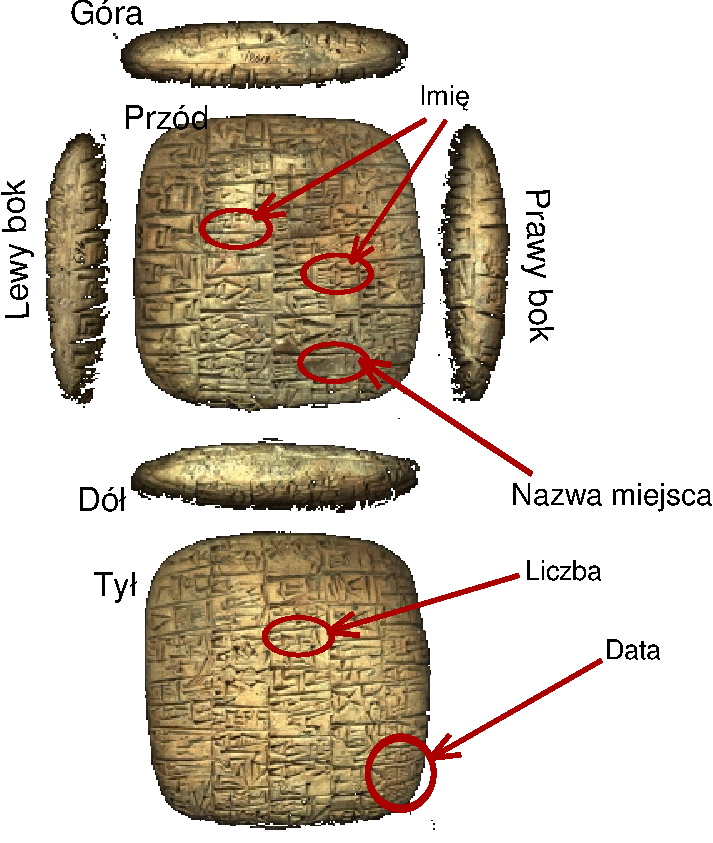
\includegraphics[bb=0 0 342 405]{./diagramy/tabliczka.pdf}
 % tabliczka.pdf: 342x405 pixel, 72dpi, 12.06x14.29 cm, bb=0 0 342 405
 \caption{Gliniana tabliczka - struktura}
\end{figure}
\begin{figure}
 \centering
 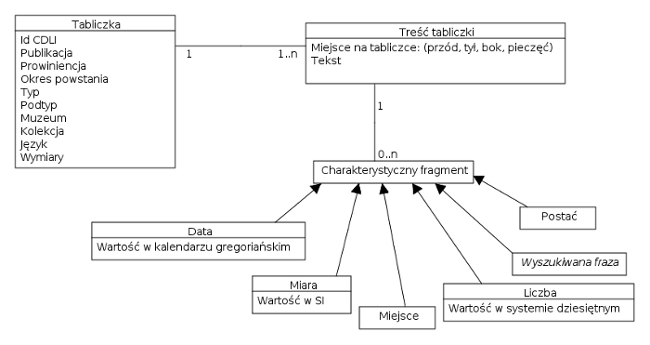
\includegraphics[width=500px,bb=0 0 650 345]{./diagramy/Model-dziedziny.png}
 % Model-dziedziny.png: 650x345 pixel, 72dpi, 22.93x12.17 cm, bb=0 0 650 345
 \caption{Co powinna zawierać tabliczka w formie elektronicznej}
\end{figure}

Głównym pojęciem jest tabliczka. Ma ona swoje metadane i treść. Tabliczka jest rozumiana dwojako - jako fizyczna tabliczka gliniana
zapisana klinami lub jako tabliczka w formie cyfrowej zapisana odczytami. Może ona zawierać elementy znaczące takie jak imię jakiejś 
osoby, liczba, jednostka (np. przy opisywaniu wypłat), miejsce, data, imię bóstwa. Część tych elementów da się przetłumaczyć na 
współczesny język (np. jednostki przeliczyć na SI, datę na datę liczbową BC). Gliniane tabliczki są zapisywane z różnych stron 
(od góry, z przodu, z tyłu itp). Poza tym zawierają pieczęcie. 

Sumerolodzy rozpoznają tabliczki po publikacjach - wiedzą mniej więcej o co chodzi jak widzą publikację.

Odczyty zawarte w cyfrowym zapisie tabliczki są wariantem tłumaczenia z klinów. W cyfrowej wersji nie ma klinów, stąd też możliwe
są pomyłki w tłumaczeniach, które ciężko zweryfikować. Są też uszkodzone fragmenty, które zostały cyfrowo zapisane w najróżniejszej
formie.

Sumerolodzy oczekują możliwości wyszukiwania po metadanych, po treści tabliczki (odczyty) i po możliwych innych tłumaczeniach (po klinach).
W pierwszej wersji języka implementujemy tylko wyszukiwanie po odczytach.
\chapter{Definicja języka TQL}
\section{Gramatyka}
\subsection{Struktura leksykalna}

\subsubsection*{String}
Literał \nonterminal{String}\ jest ciągiem dowolnych znaków w cudzysłowiu (\terminal{"} ). Nie może zawierać jedynie znaków 
``\terminal{"}`` niepoprzedzonych ''\verb6\6``.

% ma postać
% \terminal{"}$x$\terminal{"}, gdzie $x$ jest dowolnym ciągiem znaków
% poza \terminal{"}\ niepoprzedzonymi \verb6\6.


\subsubsection*{Słowo Od Litery}
Literał \nonterminal{Słowo Od Litery} to ciąg liter, cyfr oraz znaków  {''\texttt{-}``, ''\texttt{'}``, ''\texttt{\_}``}, zaczynający się od litery,
z wyjątkiem słów kluczowych.



\subsubsection*{Słowo Od Liczby}
Literał \nonterminal{Słowo Od Liczby} to ciąg liter, cyfr oraz znaków  {''\texttt{-}``, ''\texttt{'}``, ''\texttt{\_}``}, zaczynający się od cyfry.



\subsection{Słowa kluczowe}
\begin{tabular}{lll}
{\reserved{as}} &{\reserved{define}} &{\reserved{in}} \\
{\reserved{search}} & & \\
\end{tabular}\\

\subsection{Znaki specjalne}
\begin{tabular}{lll}
{\symb{(}} &{\symb{)}} &{\symb{{$+$}}} \\
{\symb{/}} &{\symb{{$-$}{$-$}}} &{\symb{*}} \\
{\symb{:}} & &{\symb{$\backslash$n}} (koniec linii)\\
\end{tabular}\\

\subsection{Komentarze}
W chwili obecnej język nie zawiera komentarzy.

\subsection{Struktura syntaktyczna języka}
Nieterminale są pomiędzy ''$\langle$`` a ''$\rangle$``. 
Symbole  ''{\arrow}``  (produkcja),  ''{\delimit}``  (lub) 
i ''{\emptyP}`` (pusta reguła) należą do notacji BNF. 
Wszystkie pozostałe symbole to terminale.\\

\begin{tabular}{lll}
{\nonterminal{Zapytanie Złożone}} & {\arrow}  &{\nonterminal{Lista Zapytań}}  \\
\end{tabular}\\

\begin{tabular}{lll}
{\nonterminal{Zapytanie}} & {\arrow}  &{\nonterminal{Lista Linii Zapytania}} {\nonterminal{Lista Pustych Linii}}  \\
 & {\delimit}  &{\terminal{define}} {\terminal{$\backslash$n}} {\nonterminal{Zapytanie}} {\terminal{as}} {\nonterminal{Nazwa}} {\nonterminal{Lista Pustych Linii}}  \\
 & {\delimit}  &{\terminal{search}} {\terminal{$\backslash$n}} {\nonterminal{Zapytanie}} {\terminal{in}} {\nonterminal{Nazwa}} {\nonterminal{Lista Pustych Linii}}  \\
 & {\delimit}  &{\nonterminal{Lista Pustych Linii}}  \\
\end{tabular}\\

\begin{tabular}{lll}
{\nonterminal{Linia Zapytania}} & {\arrow}  &{\nonterminal{Identyfikator}} {\terminal{:}} {\nonterminal{Wyrażenie}}  \\
\end{tabular}\\

\begin{tabular}{lll}
{\nonterminal{Wyrażenie}} & {\arrow}  &{\nonterminal{Wyrażenie}} {\terminal{{$+$}}} {\nonterminal{Wyrażenie1}}  \\
 & {\delimit}  &{\nonterminal{Wyrażenie}} {\terminal{/}} {\nonterminal{Wyrażenie1}}  \\
 & {\delimit}  &{\nonterminal{Wyrażenie1}}  \\
\end{tabular}\\

\begin{tabular}{lll}
{\nonterminal{Wyrażenie1}} & {\arrow}  &{\terminal{{$-$}{$-$}}} {\nonterminal{Wyrażenie1}}  \\
 & {\delimit}  &{\nonterminal{Wyrażenie2}}  \\
\end{tabular}\\

\begin{tabular}{lll}
{\nonterminal{Wyrażenie2}} & {\arrow}  &{\nonterminal{Tekst}} {\terminal{*}} {\nonterminal{Tekst}}  \\
 & {\delimit}  &{\nonterminal{Tekst}} {\terminal{*}}  \\
 & {\delimit}  &{\terminal{*}} {\nonterminal{Tekst}}  \\
 & {\delimit}  &{\nonterminal{Tekst}}  \\
 & {\delimit}  &{\terminal{(}} {\nonterminal{Wyrażenie}} {\terminal{)}}  \\
\end{tabular}\\

\begin{tabular}{lll}
{\nonterminal{Lista Zapytań}} & {\arrow}  &{\nonterminal{Zapytanie}}  \\
 & {\delimit}  &{\nonterminal{Zapytanie}} {\nonterminal{Lista Zapytań}}  \\
\end{tabular}\\

\begin{tabular}{lll}
{\nonterminal{Lista Linii Zapytania}} & {\arrow}  &{\nonterminal{Linia Zapytania}} {\terminal{$\backslash$n}}  \\
 & {\delimit}  &{\nonterminal{Linia Zapytania}} {\terminal{$\backslash$n}} {\nonterminal{Lista Linii Zapytania}}  \\
\end{tabular}\\

\begin{tabular}{lll}
{\nonterminal{Pusta Linia}} & {\arrow}  &{\terminal{$\backslash$n}}  \\
\end{tabular}\\

\begin{tabular}{lll}
{\nonterminal{Lista Pustych Linii}} & {\arrow}  &{\emptyP} \\
 & {\delimit}  &{\nonterminal{Pusta Linia}} {\nonterminal{Lista Pustych Linii}}  \\
\end{tabular}\\

\begin{tabular}{lll}
{\nonterminal{Tekst}} & {\arrow}  &{\nonterminal{String}}  \\
 & {\delimit}  &{\nonterminal{Słowo}}  \\
\end{tabular}\\


\begin{tabular}{lll}
{\nonterminal{Słowo}} & {\arrow}  &{\nonterminal{Słowo Od Litery}}  \\
 & {\delimit}  &{\nonterminal{Słowo Od Liczby}}  \\
\end{tabular}\\

\begin{tabular}{lll}
{\nonterminal{Identyfikator}} & {\arrow}  &{\nonterminal{Słowo Od Litery}}  \\
\end{tabular}\\

\begin{tabular}{lll}
{\nonterminal{Nazwa}} & {\arrow}  &{\nonterminal{String}}  \\
\end{tabular}\\

\section{Semantyka}
%możliwe pola
%W zapytaniu TQL można pytać o następujące dane:
Język TQL umożliwia wyszukiwanie na podstawie następujących danych:
\begin{longtable}{|p{3in}|p{3in}|}
\hline
{\bf Opis} & {\bf Nazwa pola w TQL}\\
\hline
\endhead
numer tabliczki w bazie CDLI & cdli\_id
\\
\hline
miejsce pochodzenia (proweniencja) & provenience
\\
\hline
okres powstania & period
\\
\hline
typ i podtyp & genre
\\
\hline
rok powstania & year 
\\
\hline
publikacja & publication
\\
\hline
treść (po odczytach)& text
\\
\hline
treść (po klinach) & cunetext
\\
\hline
kolekcja & collection
\\
\hline
muzeum & museum
\\
\hline
\end{longtable}
% \item kliny 
% \item treść na pieczęci (seal)
%  \item kod tematyczny (code)
% "provenience", "publication", "period", "year", "genre", "code", "cdli_id", "text", "seal"
Język można łatwo rozszerzać, aby umożliwić pytanie o inne dane (np. wyszukiwać po klinach czy po zawartości pieczęci).

%Semantykę przedstawimy na wybranych przykładach. 
Poniżej przedstawiamy semantykę wybranych przykładów.
\subsection{Zapytania proste}
\begin{verbatim}
provenience: Gar*
period: "Ur III"
genre: Administrative
text: udu + (masz2/ugula) --szabra
\end{verbatim}
Wynikiem zapytania będą wszystkie tabliczki, które:
\begin{itemize}
 \item pochodzą z miejscowości o nazwie zaczynającej się na ``Gar''
\item pochodzą z okresu Ur III
\item są dokumentami administracyjnymi
\item zawierają słowo ``udu'' oraz conajmniej jedno ze słów ``masz2'' lub ``ugula''
\item nie zawierają słowa ``szabra''
\end{itemize}


\subsection{Zapytania złożone}
\begin{verbatim}
provenience: Ur
period: "Ur III"/"Ur IV"
text: udu --szabra

text: masz2/ugula
publication: *tan
provenience: Ur
\end{verbatim}
Wynikiem zapytania będą wszystkie tabliczki, które:
\begin{itemize}
 \item pochodzą z miejscowości Ur
 \item pochodzą z okresu Ur III lub Ur IV
 \item zawierają słowo ``udu''
 \item nie zawierają słowa ``szabra``
\end{itemize}
oraz wszystkie tabliczki, które:
\begin{itemize}
 \item zawierają słowo ''masz2`` lub ''ugula``
 \item zostały opublikowane w pracy, której nazwa kończy się na ''tan``
 \item pochodzą z miejscowości Ur
\end{itemize}


\subsection{Zapytanie zdefiniowane}
\begin{verbatim}
 define
  provenience: Gar*a
  period: Ur III
  text: "udu ban"/mash2
as "zwierzęta w Gar*a"
\end{verbatim}
Wynikiem zapytania (po jego wywołaniu) będą wszystkie tabliczki, które:
\begin{itemize}
\item pochodzą z miejscowości, których nazwy zaczynają się na ''Gar`` i kończą na ''a''
\item pochodzą z okresu Ur III
\item zawierają conajmniej jedną z fraz ''udu ban`` lub ''mash2``
\end{itemize}

\subsection{Wywołanie zapytania zdefiniowanego}
\begin{verbatim}
search
  text: adad-tilati
in "zwierzęta w Gar*a"
\end{verbatim}
Wynikiem zapytania będą wszystkie tabliczki, które:
\begin{itemize}
 \item spełniają wszystkie warunki zapytania ''zwierzęta w Gar*a``
\item zawierają słowo ''adad-tilati``
\end{itemize}

\chapter{Implementacja}
\begin{figure}[h]
 \centering
 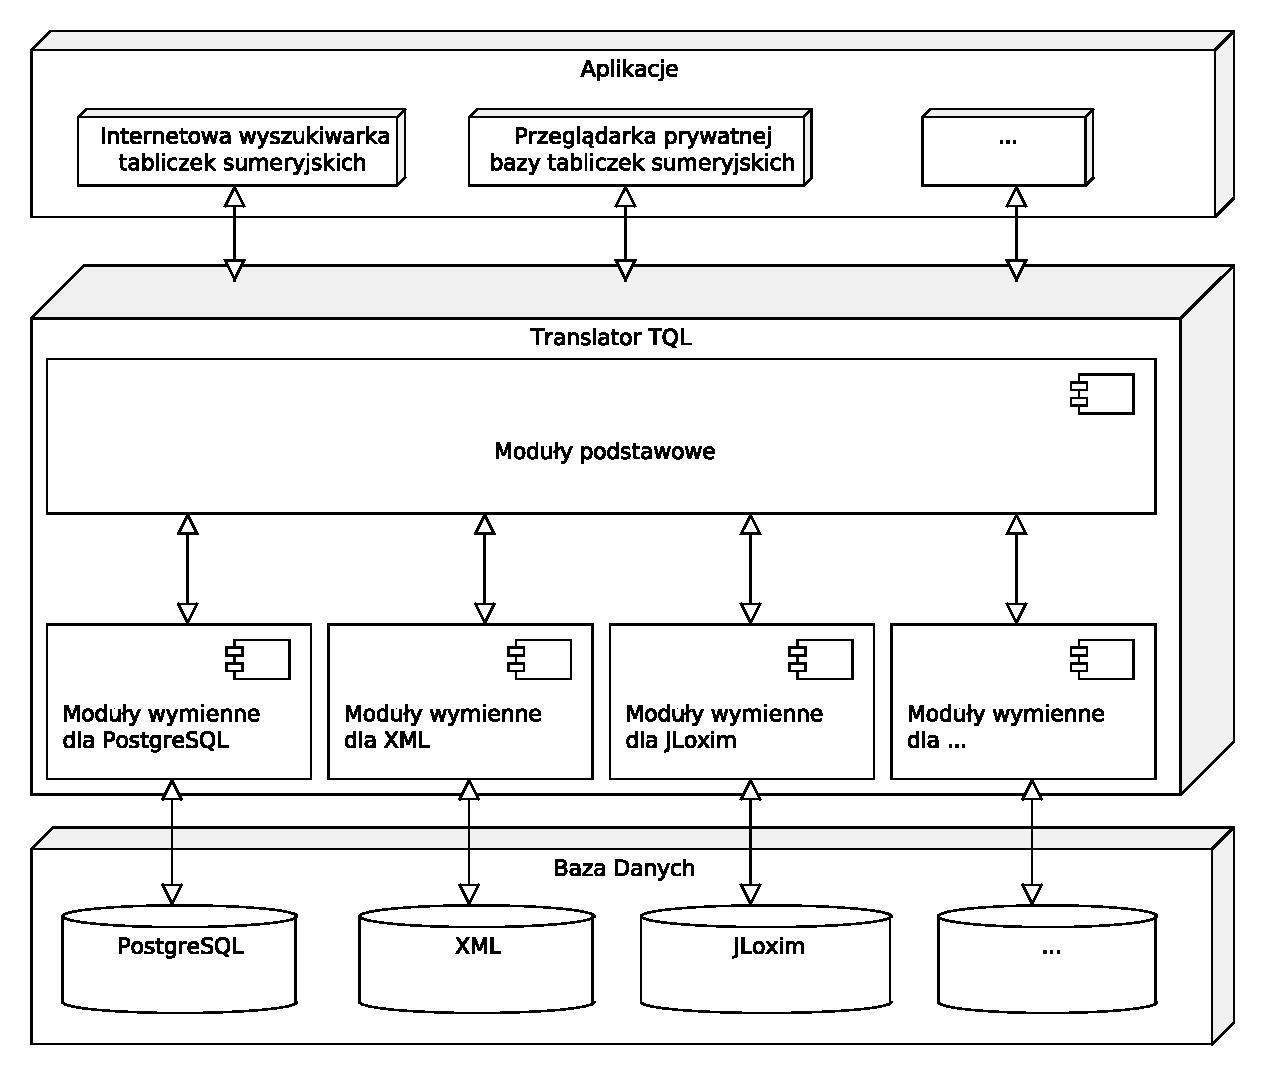
\includegraphics[width=500px,bb=0 0 608 517]{./diagramy/struktura.pdf}
 % struktura.pdf: 608x517 pixel, 72dpi, 21.45x18.24 cm, bb=0 0 608 517
 \caption{Struktura systemu korzystającego z translatora}
\end{figure}

\begin{figure}
 \centering
 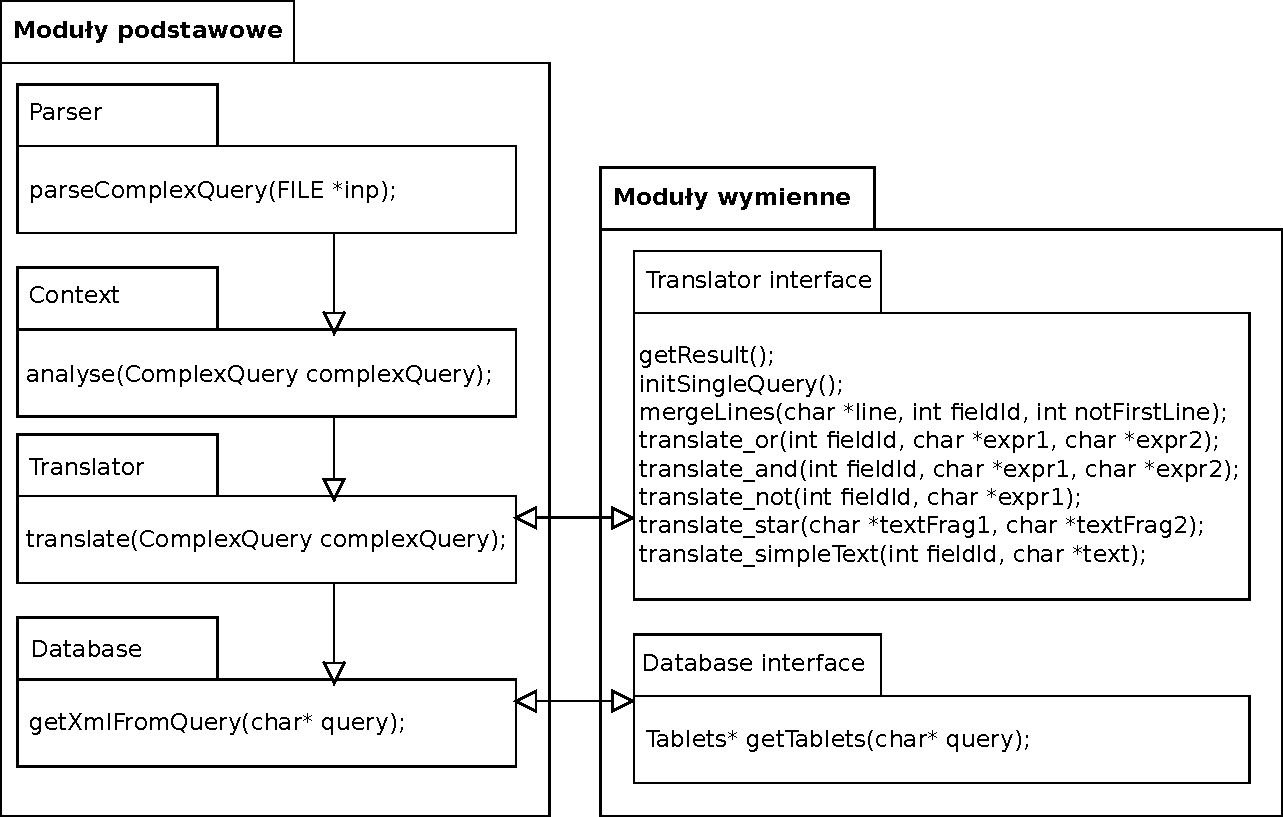
\includegraphics[width=500px,bb=0 0 585 300]{./diagramy/pakiety.pdf}
 % pakiety.pdf: 585x300 pixel, 72dpi, 20.64x10.58 cm, bb=0 0 585 300
 \caption{Podział programu na moduły}
\end{figure}
Jednym z głównych założeń języka TQL jest niezależność od struktury danych.
W związku z tym istotną cechą translatora jest możliwość dostosowania do współpracy z różnymi bazami danych.
%Jednym z głównych wymagań postawionych przed translatorem, żeby można było podłączyć różne bazy danych.
 Wynikiem tego jest podział translatora na 2 rodzaje modułów:
\begin{enumerate}
 \item \textbf{Podstawowe} -- niezależne od struktury danych i zajmujące się głównie parsowaniem i analizą składniową zapytania.
 \item \textbf{Wymienne} -- zależne od struktury danych, tłumaczące zapytanie TQL na język odpowiedni dla używanej bazy danych
i wywołujące je.
\end{enumerate}
 Wybór modułu wymiennego odbywa się na poziomie kompilacji. 
%Bez względu na wybór modułu wymiennego interfejs całego translatora jest taki sam we wszystkich instancjach.


\section{Moduły podstawowe}

\subsection{Parser}
Parser został utworzony za pomocą narzędzia BNFC. Następnie zostały w nim wprowadzone modyfikacje:
\begin{itemize}
\item poprawienie nazw stałych oznaczających symbole na bardziej intuicyjne,
\item dodanie tablicy symboli,
\item usunięcie niepotrzebnych funkcji z interfejsu,
\item uporządkowanie kodu.
\end{itemize}
Moduł ten parsuje zapytanie w języku TQL, tworząc drzewo struktury składniowej, które jest zdefiniowane w pliku pomocniczym Absyn.h.
Na parser składają się następujące pliki:
\begin{itemize}
 \item Parser.c
 \item Parser.h
 \item TQL.y % tłumaczony na Parser.c
 \item TQL.l % tłumaczony na Lexer.c
\end{itemize}

\subsection{Analizator kontekstowy}
Moduł analizuje drzewo struktury składniowej w następujący sposób:
\begin{itemize}
 \item sprawdza, czy podano prawidłowe nazwy pól,  %to co jest po lewej w linii zapytania jest nazwą pola.
\item upraszcza drzewo - z wywołania zapytania (wywołanie \textit{search in}) tworzy zapytanie proste.
\end{itemize}
Składa się z następujących plików:
\begin{itemize}
 \item Context.c
 \item Context.h
\end{itemize}

\subsection{Translator}
Zadaniem translatora jest przetłumaczenie drzewa składni abstrakcyjnej na zapytanie w docelowym języku. 
Składa się z następujących plików:
\begin {itemize}
 \item Translator.c
 \item Translator.h
 \item Translator\_config.h (interfejs modułu translatora zależnego od bazy danych)
 %\item Translator\_config.c (implementacja interfejsu z Translator\_config.h, zależny od wyboru bazy danych itp)
\end {itemize}

Tłumaczenie poszczególnych elementów drzewa zależy od implementacji interfejsu zawartego w pliku Translator\_config.h. 
Funkcja translate() przechodzi całą strukturę drzewa, wywołując w razie potrzeby odpowiednie funkcje z Translator\_config.
Następnie pobiera przetłumaczone zapytanie za pomocą funkcji getResult(), aby przekazać je do modułu bazy.

\subsection{Baza}
Moduł bazy jest odpowiedzialny za wywołanie przetłumaczonego zapytania i przekazanie wyniku w określonej formie - jako XML.
Składa się z następujących plików:
\begin {itemize}
 \item Database.c
 \item Database.h
 \item Database\_config.h (interfejs modułu bazy zależnego od bazy danych)
% \item Database\_config.c (implementacja interfejsu z Database\_conf.h, zależny od wyboru bazy danych itp)
\end {itemize}

Wywołuje funkcję getTablets() z Database\_config.h, jako parametr podając przetłumaczoną treść zapytania. 
Funkcja ta zwraca strukturę danych Tablets, wypełnioną informacjami o wyszukanych tabliczkach.
Następnie na podstawie otrzymanej struktury tworzony jest dokument XML.
\newline
Definicja struktury Tablets:
\begin{verbatim}
typedef struct{    
    char* id;
    char* id_cdli;
    char* publication;
    char* measurements;
    char* year;
    char* provenience;
    char* period;
    char* genre;
    char* subgenre;
    char* collection;
    char* text;
    Tags *tags; // specjalnie oznaczone miejsca w tekscie
                // (w pierwszej wersji frazy wyszukiwania)
} Tablet;

typedef struct{
    int size;
    Tablet *tabs;
} Tablets;
\end{verbatim}

%//miejsca gdzie w tekście są wyniki wyszukiwania

%Wszystkie niezbędne informacje powinny się znajdować w bazie danych.

\subsection{Pliki pomocnicze}
Definicje struktur danych (wygenerowane za pomocą BNFC, następnie uproszczone):
\begin{itemize}
 \item Absyn.c
\item Absyn.h
\end{itemize}
Tablica symboli:
\begin{itemize}
 \item Symbols.c
\item Symbols.h
\end{itemize}
Obsługa błędów:
\begin{itemize}
 \item Err.c
\item Err.h
\end{itemize}
Moduł do dzielenia tekstu względem separatora, pobrany z internetu \cite{cexplode}:
\begin{itemize}
 \item Cexplode.c
 \item Cexplode.h
\end{itemize}


\section{Moduły wymienne}
Pliki zależne od wyboru konkretnej bazy danych to:
\begin{itemize}
 \item Translator\_config.c - dla modułu translatora
\item Database\_config.c - dla modułu bazy
\end{itemize}
Ich interfejsy są wspólne dla wszystkich baz danych.

\subsection{Baza PostgreSQL}
\subsubsection{Diagram encji}
\begin{figure}[h]
 \centering
 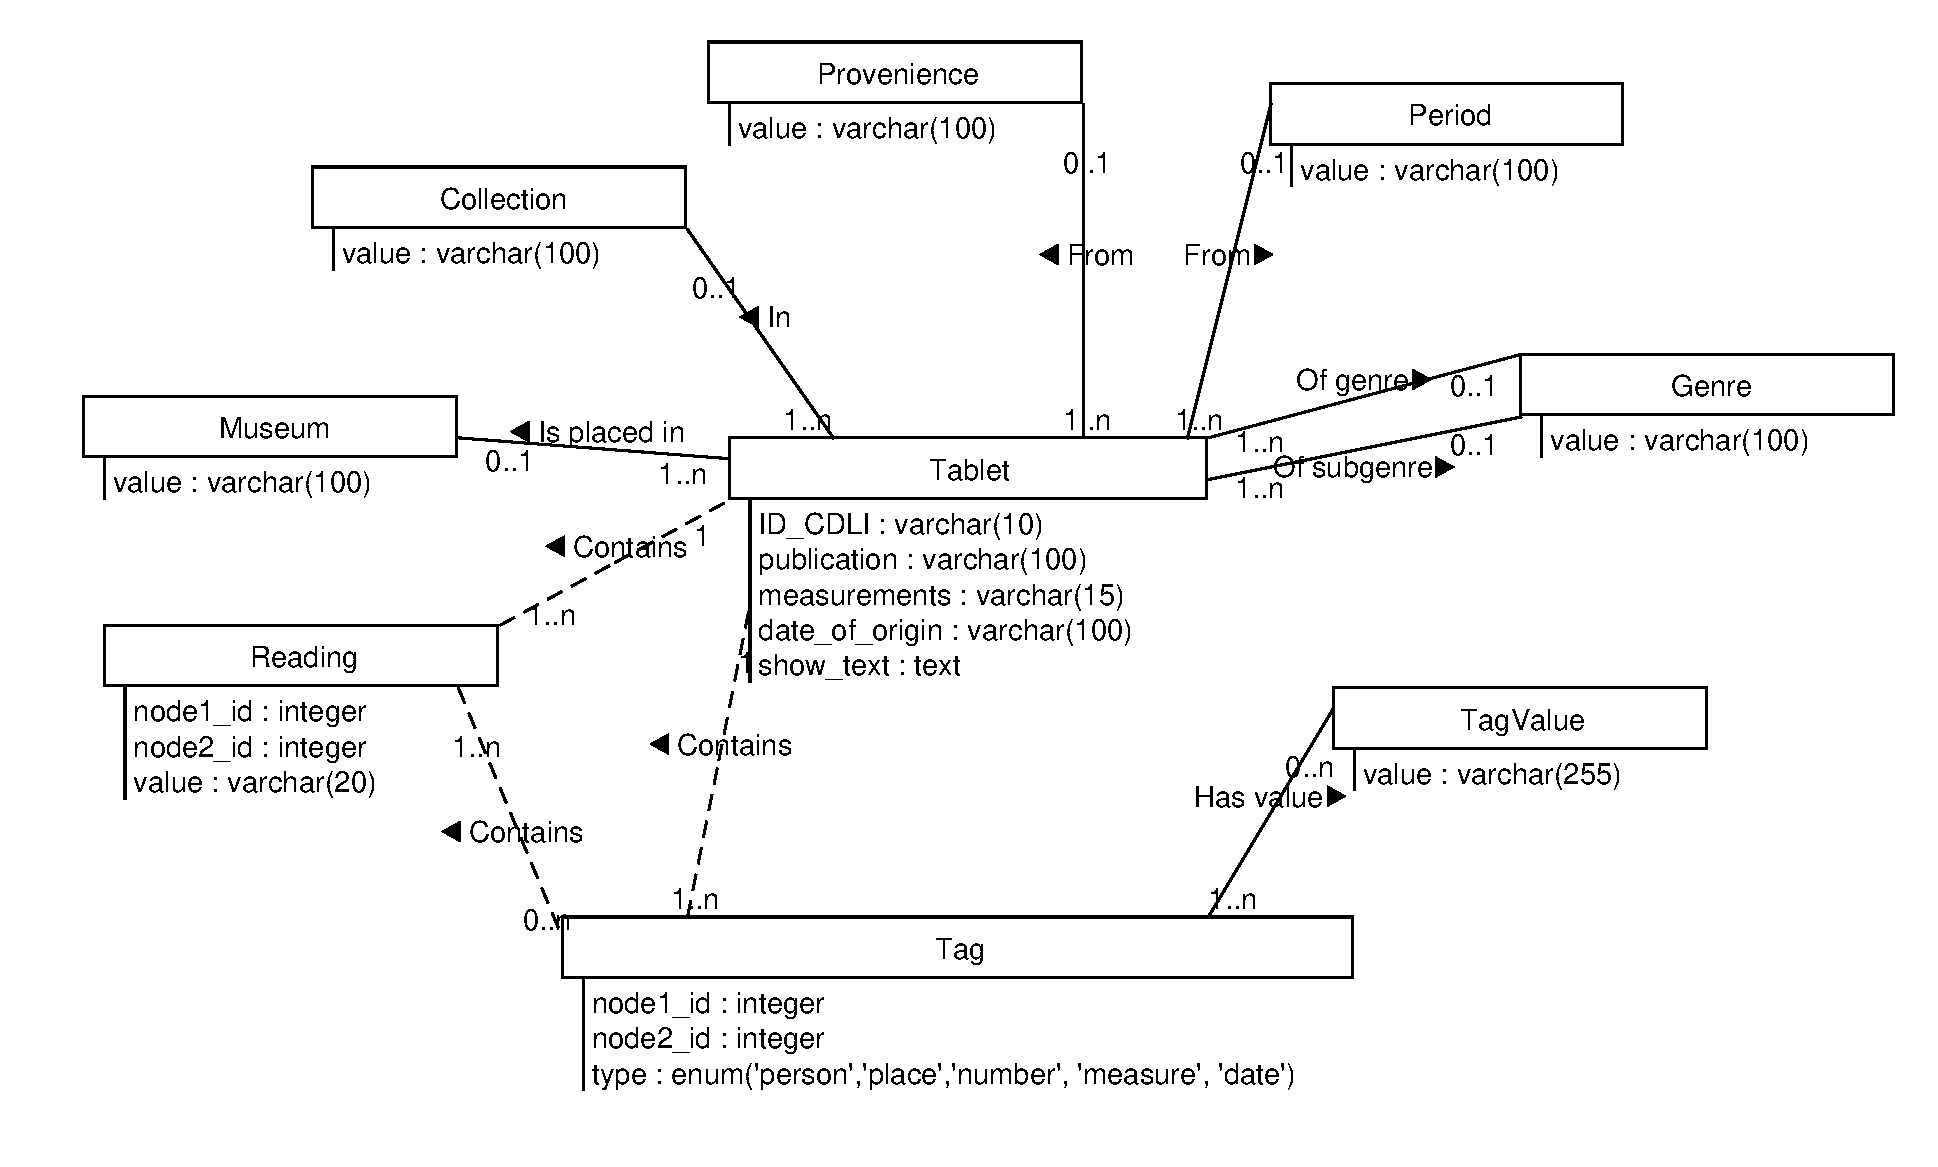
\includegraphics[width=500px,bb=0 0 930 560]{./diagramy/diagram-encji-maly.pdf}
 % diagram-encji-maly.pdf: 930x560 pixel, 72dpi, 32.81x19.76 cm, bb=0 0 930 560
 \caption{Diagram encji}
\end{figure}
Jednym z problemów przy projektowaniu bazy danych był wybór takiej reprezentacji treści tabliczki, żeby efektywnie wykonywać następujące operacje:
\begin{itemize}
 \item wyszukiwanie po treści tabliczki (po odczytach, klinach i tagach),
\item wyszukiwanie treści konkretnej tabliczki.
\end{itemize}
Najlepszym rozwiązaniem pierwszego problemu jest reprezentacja treści tabliczki
w formie grafu,
 którego krawędziami są odczyty, kliny i tagi (zgodnie z pomysłem dr Wojciecha Jaworskiego\cite[s.13-24]{jaworski}).
Natomiast w przypadku drugiego problemu narzuca się przechowywanie treści
jako otwarty tekst.
Zdecydowałyśmy się na połączenie obu sposobów. Odczyty, kliny i tagi przechowujemy w tabelach Reading, Cuneiform i Tag, 
natomiast otwarty tekst w kolumnie show\_text tabeli Tablet.
Aby zapewnić możliwość odwzorowania treści tabliczki między reprezentacjami, węzły są liczbami postaci:
%Treść tabliczki jest przechowywana nie tylko jako otwarty tekst (kolumna w tabeli Tablet), ale także w formie grafu,
 %którego krawędziami są odczyty i tagi (zgodnie z pomysłem dr Wojciecha Jaworskiego\cite[s.13-24]{jaworski}) 
%w tabelach Reading i Tag. 
%  Węzeł tego grafu jest liczbą postaci:
\begin{verbatim}
 <numer węzła w tabliczce> * 1 000 000 + <id tabliczki>
\end{verbatim}
gdzie numer węzła w tabliczce to numer kolejnego słowa (słowa są oddzielone spacjami i końcem linii) pomnożone przez 10 (żeby umożliwić
wstawienie kilku węzłów w jednym słowie np. pozwolić na przetłumaczenie jednego słowa na sekwencję trzech klinów). 


Przerywane linie na diagramie encji oznaczają opisany powyżej związek pomiędzy id węzła (node1\_id i node2\_id) 
a id tabliczki (Tablet.id).

% relacja
% Stąd wzięły się przerywane linie na diagramie encji - nie ma bezpośredniego klucza obcego w tabeli Reading (czy Tag) do Tablet, 
% jednak związek istnieje. Taki sposób przechowywania informacji o treści tabliczki umożliwia sprawniejsze wyszukiwanie nie tylko
% po odczytach (pozwala pomijać linie z uszkodzeniami) ale także w przyszłości ułatwia zaimplementowanie wyszukiwania po klinach,
% po tagach itp.
% Poza sprawnym
%  wyszukiwaniem ułatwia to rozszerzenie programu o możliwość wyszukiwania po klinach - po dodaniu tabeli Cuneiform.

 

\subsubsection{Translator\_config}
Tłumaczy otrzymane fragmenty drzewa struktury zapytania na język SQL. Przetłumaczone fragmenty zbiera do buforów 
(\textit{select}, \textit{from}, \textit{where}), które następnie odpowiednio łączy.
Każde proste zapytanie TQL jest tłumaczone na pojedyncze zapytanie SQL. Tłumaczenie kilku prostych zapytań
łączone jest za pomocą UNION.

\subsubsection{Inicjalizacja zapytania}
Tłumaczenie prostego zapytania zaczyna się od inicjalizacji buforów przechowujących poszczególne części wynikowego SQL-a.
\textit{select} jest inicjowany na 
\begin{verbatim}
SELECT t.id, t.id_cdli, t.publication, t.measurements, t.origin_date, 
       p.value as provenience, pd.value as period,
       g1.value as genre, g2.value as subgenre, 
       c.value as collection, t.text
\end{verbatim}
\textit{from} jest inicjowany
\begin{verbatim}
FROM tablet t
  LEFT JOIN provenience p ON p.id=t.provenience_id
  LEFT JOIN collection c ON c.id=t.collection_id
  LEFT JOIN genre g1 ON g1.id=t.genre_id
  LEFT JOIN genre g2 ON g2.id = t.subgenre_id
  LEFT JOIN period pd ON pd.id = t.period_id
\end{verbatim}
\textit{where} początkowo zawiera pusty ciąg znaków.



\subsubsection{Tłumaczenie konstrukcji prostych}
Poniższe tłumaczenia są dodawane do bufora \textit{where} i łączone za pomocą AND.
\begin{longtable}{|p{3in}|p{3in}|}
\hline
{\bf Konstrukcja} & {\bf Tłumaczenie na SQL}\\
\hline
\endhead
provenience: wartosc & \begin{verbatim}p.value LIKE 'wartosc'\end{verbatim}
\\
\hline
publication: wartosc & 
\begin{verbatim}
t.publication LIKE 'wartosc'
\end{verbatim}
\\
\hline
period: wartosc & 
\begin{verbatim}
pd.value LIKE 'wartosc'
\end{verbatim}
\\
\hline
year: wartosc & 
\begin{verbatim}
t.origin_date LIKE 'wartosc'
\end{verbatim}
\\
\hline
genre: wartosc & 
\begin{verbatim}
   g1.value LIKE 'wartosc' 
OR g2.value LIKE 'wartosc'
\end{verbatim}
\\
\hline
cdli\_id: wartosc & 
\begin{verbatim}
t.cdli_id LIKE 'wartosc'
\end{verbatim}
\\
\hline
museum: wartosc & 
\begin{verbatim}
t.museum LIKE 'wartosc'
\end{verbatim}
\\
\hline
collection: wartosc & 
\begin{verbatim}
c.value LIKE 'wartosc'
\end{verbatim}
\\
\hline
\end{longtable}

\textbf{Tłumaczenie operatorów:}
\begin{longtable}{|p{1in}|p{1in}|}
\hline
{\bf Operator} & {\bf Tłumaczenie}\\
\hline
\endhead
/ & OR\\ 
\hline
-- & NOT\\ 
\hline
+ & AND\\ 
\hline
* & \%  \\ 
\hline
\end{longtable}


\subsubsection{Tłumaczenie konstrukcji złożonych}
%Została zaimplementowana tylko jedna konstrukcja złożona - przy zapytaniu o treść tabliczki (pole ''text``).
Przy tłumaczeniu konstrukcji złożonych
korzystamy z przedstawienia treści tabliczki w formie grafu.

Pojawienie się wyszukiwania po treści tabliczki niesie za sobą konieczność dodania do bufora \textit{from}:
\begin{verbatim}
INNER JOIN (
  <wynikowe zapytanie o treść tablczki>
) AS sequence ON sequence.id_tab = t.id
\end{verbatim}

natomiast do \textit{select} dodajemy:
\begin{verbatim}
, sequence.nodes as nodes
\end{verbatim}

gdzie $<$wynikowe zapytanie o treść tablczki$>$ to kombinacja zapytań typu:
\begin{verbatim}
  SELECT 
    id_tab, 
    CAST(array_accum(nodes) as TEXT) as nodes, 
    COUNT(DISTINCT id_seq) AS seq, 
    <id_seq> AS id_seq
  FROM (
    SELECT
      t1.node1_id % 1000000 AS id_tab,
      '{' || t1.node1_id || ',' || t<dl_sekw>.node2_id || '}' AS nodes,
      1 AS id_seq
    FROM
      <nazwa_tabeli> t1
      LEFT JOIN <nazwa_tabeli> t2 ON (t2.node1 = t1.node2)
      LEFT JOIN <nazwa_tabeli> t3 ON (t3.node1 = t2.node2)
      ...
      LEFT JOIN <nazwa_tabeli> t<dl_sekw> ON (t<dl_sekw>.node1 = t<dl_sekw-1>.node2)
   WHERE
      t1.value LIKE '<sekw[1]>'
     AND
      t2.value LIKE '<sekw[2]>'
    AND
      t3.value LIKE '<sekw[3]>'
    AND
      ...
    AND
      t<dl_sekw>.value LIKE '<sekw[<dl_sekw>]>'
   ) AS a 
  GROUP BY id_tab
\end{verbatim}
Zmienne użyte w powyższym pseudo-kodzie:
\begin{description}
 \item[id\_sekw] - kolejny numer sekwencji (przydatny przy bardziej skomplikowanym zapytaniu - do rozróżniania podzapytań)
 \item[dl\_sekw] - ilość słów składających się na wyszukiwaną sekwencję
 \item[sekw] - tablica zawierająca słowa składające się na wyszukiwaną sekwencję
\item[nazwa\_tabeli] - nazwa tabeli, w której wyszukujemy (Reading lub Cuneiform)
 \end{description}

\begin{longtable}{|p{1in}|p{4.5in}|}
\hline
{\bf Operator} & {\bf Tłumaczenie}\\
\hline
\endhead
/ & 
\begin{verbatim}
SELECT 
  id_tab, 
  CAST(array_accum(nodes) as TEXT) as nodes, 
  COUNT(DISTINCT id_seq) as seq,
  <id_sekw> as id_seq
FROM 
(
  <zapytanie1>
  UNION
  <zapytanie2>
)
as c
GROUP BY id_tab
\end{verbatim}
\\ 
\hline
+ &
\begin{verbatim}
SELECT * FROM
 (SELECT id_tab, 
         CAST(array_accum(nodes) as TEXT) as nodes, 
         COUNT(DISTINCT id_seq) as seq, 
         <id_sekw> as id_seq
  FROM
    (<zapytanie1>
    UNION
    <zapytanie2>)
  as c 
  GROUP BY id_tab
 ) as b
WHERE b.seq=2 
\end{verbatim}
\\ 
\hline
-- & 
\begin{verbatim}
SELECT 
  id_tab, 
  '' as wezly, 
  0 as sekw,
  <id_sekw> as id_sekw
FROM
(
 (SELECT id as id_tab from tabliczka)
 EXCEPT
 (SELECT id_tab from
    <zapytanie_negowane> as a
 )   
) as b
\end{verbatim}
\\ 
\hline
* & \%  \\ 
\hline
\end{longtable}


\subsubsection{Database\_config}

Odpowiada za wywołanie zapytania na konkretnej bazie i zapisanie wyniku do struktury Tablets.
 Korzysta z pliku database.conf, który zawiera dane dostępu do bazy (host, port, użytkownik, hasło, nazwa bazy)
oraz biblioteki libpq-fe.h do PostgreSQL.

\subsection{Baza XML}
W budowie :)
%\chapter{Dokumentacja użytkowa i opis implementacji}\label{r:impl}

\chapter{Podsumowanie}


\appendix



\begin{thebibliography}{99}
\addcontentsline{toc}{chapter}{Bibliografia}
\bibitem[1]{jaworski} Wojciech Jaworski, \textit{Modelowanie tresci sumeryjskich tekstów gospodarczych z epoki Ur~III}, 
\url{http://nlp.ipipan.waw.pl/NLP-SEMINAR/071119.pdf}, 19 listopada 2007
\bibitem[2]{cexplode} \url{http://maz-programmersdiary.blogspot.com/2008/09/c-explode.html}



%\bibitem[Bea65]{beaman} Juliusz Beaman, \textit{Morbidity of the Jolly
 %   function}, Mathematica Absurdica, 117 (1965) 338--9.

\end{thebibliography}

\listoffigures

\end{document}


%%% Local Variables:
%%% mode: latex
%%% TeX-master: t
%%% coding: latin-2
%%% End:
